\documentclass[]{report}

\usepackage{circuitikz}
\usepackage{amsmath}
\usepackage{tikz}
\usepackage{tikzsymbols}
\usepackage{pgfplots}
\usepackage{layout}
\usepackage[left=25mm, right=25mm]{geometry}

\pgfplotsset{compat=1.18}

\DeclareMathOperator{\sech}{sech}
\DeclareMathOperator{\csch}{cosech}

\newcommand{\vct}{\boldsymbol}
\newcommand{\unt}{\hat}

\begin{document}

\title{Calculus}
\author{Jack Thomas}
\date{}

\maketitle
\newpage

\tableofcontents
\newpage 
\part{Single Variable Calculus}

\chapter{Differentiation}
\section{The Derivative}

The derivative measures change. More specifically, if we have a function, f(x), then the derivative
of this function (often denoted f'(x)) tells us how quickly the function is increasing or decreasing
at any given point. If we consider a general function and think how we might measure how it changes,
we may look at the difference in the function between two values of x.

\begin{center}
    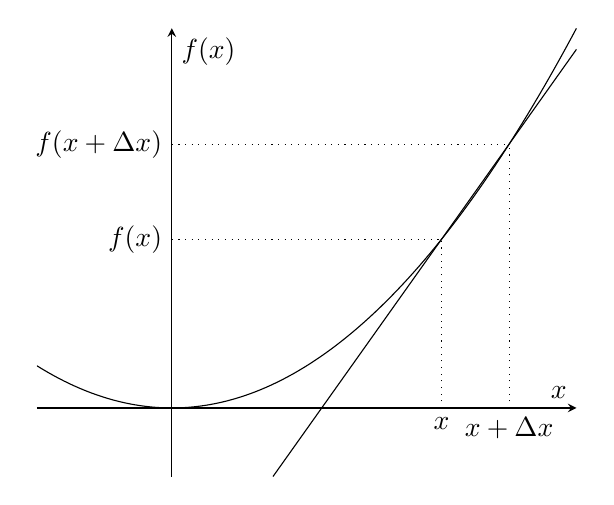
\begin{tikzpicture}[scale=1]
    \begin{axis}[
        axis lines = left,
        axis lines = center,
        xtick style={draw=none},
        ytick style={draw=none},
        xticklabels={},
        yticklabels={},
        xlabel = {$x$},
        ylabel = {$f(x)$},
    ]
    
    \node [left] at (0, 64) {\(f(x)\)};
    \node [left] at (0, 100) {\(f(x + \Delta x)\)};
    \node [below] at (8, 0) {\(x\)};
    \node [below] at (10, 0) {\(x + \Delta x\)};
    \addplot [
        domain=-4:12, 
        samples=100, 
        color=black,
    ]
    {x^2};
    \addplot+ [
        black, dotted,
        mark=none,
    ]
    coordinates {
        (8,0)
        (8,64)

        (10,0)
        (10,100)

        (0, 64)
        (8, 64)

        (0, 100)
        (10, 100)

    };
    \addplot+ [
        black,
        mark=none
    ]
    coordinates {
        (3,-26)
        (12, 136)
    };
    \end{axis}
    \end{tikzpicture}
\end{center}

Here we have two points, one at $x = x_1$ and $x = x_2 = x_1 + \Delta x$. Here $\Delta$ means "change in"
and so $\Delta x$ denotes the difference between our two x values. The corresponding function values are
$f(x_1)$ and $f(x_1 + \Delta x)$ where the difference between these two values is $\Delta f$. We can say 
a reasonable estimate of the rate of change would be the gradient of the line that passes through these two 
points. We can write this as

\begin{equation} \label{gradient}
    \frac{\Delta f}{\Delta x} = \frac{f(x + \Delta x) - f(x)}{\Delta x}
\end{equation}

We can see that this estimate for the rate of change gets better the closer the two points are, or the smaller 
$\Delta x$ gets. If we take the limit of $\Delta x \to 0$, then our two points become infinitesimally close and the
line through them becomes the tangent line to the curve. Thus we arrive at the definition of the derivative and the
idea of "instantaneous" rate of change. The derivative is defined as a function which gives us the gradient of the 
tangent line to a curve at a point $x$. Mathematically we can write this as

\begin{equation*}
    f'(x) \equiv \frac{df}{dx} \equiv \lim_{\Delta x \to 0} \frac{\Delta f}{\Delta x}\\
\end{equation*}

Using the expression for the gradient above we then get

\begin{equation} \label{deriv-def}
    \frac{df}{dx} \equiv \lim_{\Delta x \to 0} \frac{f(x + \Delta x) - f(x)}{\Delta x}
\end{equation}

Which is our formal definition of the derivative. The process of finding a functions derivative is called 
differentiation. We can differentiate from first principles using the expression above.\\

\noindent\textbf{Example: Differentiate the function $x^2$ using first principles.}

Using equation \ref{deriv-def}, we have that

\begin{align*}
    \frac{d}{dx}(x^2) &= \lim_{\Delta x \to 0} \frac{(x + \Delta x)^2 - x^2}{\Delta x}\\
    &= \lim_{\Delta x \to 0} \frac{(x^2 + 2x\Delta x + \Delta x^2) - x^2}{\Delta x}\\
    &= \lim_{\Delta x \to 0} \frac{2x\Delta x + \Delta x^2}{\Delta x}\\
    &= \lim_{\Delta x \to 0} 2x + \Delta x\\
    &= 2x\\
\end{align*}

We can generalise the above example differentiating $x^n$ instead. With which we get

\begin{align*}
    \frac{d}{dx}(x^{n}) &= \lim_{\Delta x \to 0} \frac{(x + \Delta x)^{n} - x^{n}}{\Delta x}\\
    &= \lim_{\Delta x \to 0} \frac{(x^{n} + n x^{n-1}\Delta x + \binom{n}{2}x^{n-2}\Delta x^{2} +\dots) - x^{n}}{\Delta x}\\
    &= \lim_{\Delta x \to 0} \frac{n x^{n-1}\Delta x + \binom{n}{2}x^{n-2}\Delta x^{2}}{\Delta x} + \dots\\
    &= \lim_{\Delta x \to 0} n x^{n-1} + \binom{n}{2}x^{n-2}\Delta x + \dots\\
    &= n x^{n-1}
\end{align*}

We know this is true for all $n$ as any subsequent terms will contain a factor of $\Delta x$ which 
follows from the binomial theorem. The expression we have just derived is known as the power rule
which we can use to differentiate any power term. There are further rules of differentiation which
will allow us to differentiate any function thrown at us.

\begin{equation*}
    \frac{d}{dx}(e^{ax}) = ae^{ax}
\end{equation*}

\section{The Chain Rule}

The first rule is the chain rule which we use to differentiate composite functions, or "functions
of functions"

\begin{equation*}
    \frac{d}{dx}f[g(x)] = \frac{df}{dg} \frac{dg}{dx}
\end{equation*}

\section{The Product Rule}

\begin{equation*}
    \frac{d}{dx} \left[f(x)g(x)\right] = \frac{df}{dx} g(x) + f(x)\frac{dg}{dx}
\end{equation*}

\begin{equation*}
    (uv)' = u' v + uv'
\end{equation*}

\begin{equation*}
    \frac{d}{dx} \left[f(x)g(x)h(x)\right] = \frac{df}{dx} g(x)h(x) + f(x)\frac{dg}{dx} h(x) + f(x)g(x) \frac{dh}{dx}
\end{equation*}

\begin{align*}
    \frac{d}{dx}\left(\frac{f(x)}{g(x)}\right) &= \frac{df}{dx}\left(\frac{1}{g(x)}\right) + f(x)\frac{d}{dx}\left(\frac{1}{g(x)}\right)\\
    &= \frac{f'(x)}{g(x)} + f(x)\left(- \frac{g'(x)}{(g(x))^2}\right)\\
    &= \frac{f'(x)}{g(x)} - \frac{f(x)g'(x)}{(g(x))^{2}}\\
    &= \frac{f'(x)g(x) - f(x)g'(x)}{(g(x))^{2}}
\end{align*}

\section{Implicit Differentiation}
\chapter{Integration}
\section{The Antiderivative}

\begin{equation*}
    I = \int_{a}^{b} f(x)dx
\end{equation*}

\begin{equation*}
    \int x^{n}dx = \frac{x^{n+1}}{n+1} + C
\end{equation*}

\[\int e^{ax}dx = \frac{1}{a}e^{ax} + c, \qquad \int \frac{1}{x}dx = ln(x) + c\]

\section{Integration by Substitution}
\section{Integration by Parts}

\begin{equation*}
    \frac{d}{dx}(uv) = u \frac{dv}{dx} + \frac{du}{dx} v
\end{equation*}

\begin{equation*}
    uv = \int u \frac{dv}{dx} dx + \int \frac{du}{dx}vdx
\end{equation*}
    
\begin{equation*}
    \int u \frac{dv}{dx} dx = uv - \int \frac{du}{dx}vdx
\end{equation*}

\section{Surfaces and Volumes of Revolution}

\begin{equation*}
    \Delta S \approx \sqrt{(\Delta x)^{2} + (\Delta y)^{2}}
\end{equation*}

\begin{equation*}
    S = \int_{a}^{b} 2 \pi y ds
\end{equation*}

\begin{equation*}
    S = \int_{a}^{b} 2 \pi y \sqrt{1 + \left(\frac{dy}{dx}\right)^{2}}dx
\end{equation*}

\begin{equation*}
    V = \int_{a}^{b} \pi y^{2} dx
\end{equation*}

\section{Plane Polar Coordinates}
\chapter{Series}

\section{Power Series}

\section{Taylor Series}

\begin{equation*}
    f(x) = a_0 + a_1 x + a_2 x^2 + a_3 x^3 + \dots = \sum_{n}^{\infty}a_n x^n
\end{equation*}

\begin{equation*}
    f'(x) = a_1 + 2a_2 x + 3a_3 x^2 + \dots = \sum_{n}^{\infty}n a_n x^{n-1}
\end{equation*}

\begin{equation*}
    f''(x) = \sum_{n}^{\infty} n(n-1) a_n x^{n-2}
\end{equation*}

\begin{equation*}
    f(x) = f(a) + (x-a)f'(a) + \frac{(x-a)^2}{2!}f''(a) + 
\end{equation*}

\begin{equation*}
    \sin(x) = x - \frac{x^{3}}{3!} + \frac{x^{5}}{5!} - \frac{x^{7}}{7!} + \dots
\end{equation*}

\begin{equation*}
    \cos(x) = 1 - \frac{x^{2}}{2!} + \frac{x^{4}}{4!} - \frac{x^{6}}{6!} + \dots
\end{equation*}

\begin{equation*}
    e^{x} = 1 + \frac{x^{2}}{2!} + \frac{x^{3}}{3!} + \frac{x^{4}}{4!} + \dots
\end{equation*}

\section{ L’Hopital's Rule}
\chapter{Complex Numbers}

\section{Imaginary Numbers}
\begin{equation*}
    i = \sqrt{-1}
\end{equation*}

\begin{equation*}
    z = x + iy
\end{equation*}

\begin{align*}
    e^{i\theta} &= 1 + i\theta + \frac{(i\theta)^{2}}{2!} + \frac{(i\theta)^{3}}{3!} + \frac{(i\theta)^{4}}{4!}\\
    &= 1 + i\theta - \frac{\theta^{2}}{2!} - \frac{i\theta^{3}}{3!} + \frac{\theta^{4}}{4!} + \dots\\
    &= \left(1 - \frac{\theta^{2}}{2!} + \frac{\theta^{4}}{4!} + \dots\right) + i\left(\theta - \frac{i\theta^{3}}{3!} + \frac{i\theta^{5}}{5!} + \dots\right)
\end{align*}

\begin{equation*}
    e^{i\theta} = \cos\theta + i\sin\theta
\end{equation*}

\section{De Moivre's Theorem}

\begin{equation*}
    e^{in\theta} = \cos n\theta + i \sin n\theta
\end{equation*}

\section{Hyperbolic Functions}

\begin{equation*}
    \cosh(x) = \frac{1}{2}(e^x + e^{-x})
\end{equation*}

\begin{equation*}
    \sinh(x) = \frac{1}{2}(e^x - e^{-x})
\end{equation*}

\part{Multi Variable Calculus}

\chapter{Partial Differentiation}

\section{The Partial Derivative}

\begin{equation*}
    \frac{\partial f}{\partial x} = \lim_{\Delta x \to 0}\frac{f(x + \Delta x, y) - f(x, y)}{\Delta x}
\end{equation*}

\begin{equation*}
    \frac{\partial f}{\partial y} = \lim_{\Delta y \to 0}\frac{f(x, y + \Delta y) - f(x, y)}{\Delta y}
\end{equation*}

\[\frac{\partial}{\partial x}\left(\frac{\partial f}{\partial x}\right) = \frac{\partial^{2}f}{\partial x ^{2}} \qquad \frac{\partial}{\partial y}\left(\frac{\partial f}{\partial y}\right) = \frac{\partial^{2}f}{\partial y ^{2}}\]

\begin{equation*}
    \frac{\partial^{2}f}{\partial x \partial y} = \frac{\partial^{2}f}{\partial y \partial x}
\end{equation*}

\section{The Total Differential}

\begin{equation*}
    \Delta f \approx \frac{\partial f(x, y)}{\partial x}\Delta x + \frac{\partial f(x, y)}{\partial y}\Delta y
\end{equation*}

\begin{equation*}
    df = \frac{\partial f(x, y)}{\partial x}dx + \frac{\partial f(x, y)}{\partial y}dy
\end{equation*}

\begin{equation*}
    df = \sum_{i}^{n}\frac{\partial f}{\partial x_{i}}dx_{i}
\end{equation*}

\begin{equation*}
    \frac{df}{dx_{1}} = \sum_{i}^{n}\left(\frac{\partial f}{\partial x_{i}}\right)\frac{dx_{i}}{dx_{1}}
\end{equation*}

\section{Exact Differentials}

\begin{equation*}
    df = A(x, y)dx + B(x, y)dy
\end{equation*}

\begin{equation*}
    \frac{\partial f}{\partial x} = A(x, y), \qquad \frac{\partial f}{\partial y} = B(x, y)
\end{equation*}

\begin{equation*}
    \frac{\partial A}{\partial x} = \frac{\partial B}{\partial x}
\end{equation*}

\section{Change of Variables}

\section{Maxima and Minima}

\begin{equation*}
    \frac{\partial f}{\partial x} = 0, \qquad \frac{\partial f}{\partial y} = 0
\end{equation*}

\section{Lagrange Multipliers}

\section{Leibnitz' Rule}

\begin{equation*}
    F(x,t) = \int f(x,t)dt
\end{equation*}

\begin{equation*}
    \frac{\partial F(x,t)}{\partial x} = f(x,t)
\end{equation*}

\begin{equation*}
    \frac{\partial^{2}F(x,t)}{\partial t \partial x} = \frac{\partial^{2}F(x,t)}{\partial x \partial t}
\end{equation*}

\begin{equation*}
    \frac{\partial}{\partial t}\left[\frac{\partial F(x,t)}{\partial x}\right] =
    \frac{\partial}{\partial x}\left[\frac{\partial F(x,t)}{\partial t}\right] =
    \frac{\partial f(x,t)}{\partial x}
\end{equation*}

\begin{equation*}
    \frac{\partial F(x,t)}{\partial x} = \int \frac{\partial f(x,t)}{\partial x} dt
\end{equation*}

\begin{align*}
    I(x) &= \int_{t=v}^{t=u}f(x,t)dt\\
    &= F(x,v) - F(x,u)
\end{align*}

\begin{align*}
    \frac{dI(x)}{dx} &= \frac{\partial F(x,v)}{\partial x} - \frac{\partial F(x,u)}{\partial x}\\
    &= \int^{v} \frac{\partial f(x,t)}{\partial x}dt - \int^{u} \frac{\partial f(x,t)}{\partial x}dt\\
    &= \int_{u}^{v} \frac{\partial f(x,t)}{\partial x}dt
\end{align*}

\begin{align*}
    I(x) &= \int_{t=v(x)}^{t=u(x)}f(x,t)dt\\
    &= F(x,v(x)) - F(x,u(x))
\end{align*}
\chapter{Multiple Integrals}

\section{Double Integrals}

\begin{equation*}
    I = \int_{}^{}f(x,y)dA
\end{equation*}

\begin{equation*}
    I = \int_{}^{}\int_{}^{}f(x,y)dxdy
\end{equation*}

\begin{equation*}
    I = \int_{y=c}^{y=d}\left\{
        \int_{x=x_1(y)}^{x=x_2(y)}
        f(x, y)dx
    \right\}dy
\end{equation*}

\section{Triple Integrals}

\begin{equation*}
    I = \int_{}^{}f(x,y,z)dV
\end{equation*}

\begin{equation*}
    I = \int_{}^{}\int_{}^{}f(x,y)dxdydz
\end{equation*}

\begin{equation*}
    I = \int_{x_1}^{x_2}dx
    \int_{y_1(x)}^{y_2(x)}dy
    \int_{z_1(x,y)}^{z_2(x,y)}f(x,y,z)dz
\end{equation*}

\section{Change of Variables and The Jacobian}

\begin{equation*}
    dA_{uv} = 
    \begin{vmatrix}
        \dfrac{\partial x}{\partial u}du
        \dfrac{\partial y}{\partial v}dv - 
        \dfrac{\partial x}{\partial v}dv
        \dfrac{\partial y}{\partial u}du
    \end{vmatrix}
\end{equation*}

\begin{equation*}
    J \equiv \frac{\partial (x,y)}{\partial (u,v)} \equiv 
    \frac{\partial x}{\partial u}\frac{\partial y}{\partial v} -
    \frac{\partial x}{\partial v}\frac{\partial y}{\partial u}
\end{equation*}

\begin{equation*}
    J =
    \begin{vmatrix}
        \dfrac{\partial x}{\partial u} & \dfrac{\partial y}{\partial v} \\[2ex]
        \dfrac{\partial x}{\partial v} & \dfrac{\partial y}{\partial u} \\
    \end{vmatrix}
\end{equation*}

\section{The Gaussian Integral}

\chapter{Vector Algebra}

\section{Vector Operations}

\begin{equation*}
    \vct{a}  + \vct{b} = \vct{b} + \vct{a}
\end{equation*}

\begin{equation*}
    \vct{a} + (\vct{b} + \vct{c}) = (\vct{a} + \vct{b}) + \vct{c}
\end{equation*}

\begin{equation*}
    \vct{a} -  \vct{b} =  \vct{a} +(- \vct{b})
\end{equation*}

\subsection*{Scalar Multiplication}

\begin{align*}
    (\lambda\mu)\vct{a} &= \lambda(\mu\vct{a}) = \mu(\lambda\vct{a})\\
    \lambda(\vct{a} +  \vct{b}) &= \lambda\vct{a} + \lambda\vct{b} \\
    (\lambda + \mu)\vct{a} &= \lambda\vct{a} + \mu\vct{a} 
\end{align*}

\section{Basis Vectors}

\begin{equation*}
    \vct{a} = a_1\vct{e}_1 + a_2\vct{e}_2 + a_3\vct{e}_3
\end{equation*}

\begin{equation*}
    \vct{\unt{a}} = \frac{\vct{a}}{|\vct{a}|}
\end{equation*}

\begin{equation*}
    a \equiv |\vct{a}| = \sqrt{a_x^2 + a_y^2 + a_z^2}
\end{equation*}

\begin{equation*}
    \vct{a} = a_x\vct{\unt{x}} + a_y\vct{\unt{y}} + a_z\vct{\unt{z}}
\end{equation*}

\begin{equation*}
    \vct{a} \pm \vct{b} =
    (a_x \pm b_x)\vct{\unt{x}} + 
    (a_y \pm b_y)\vct{\unt{y}} + 
    (a_z \pm b_z)\vct{\unt{z}}
\end{equation*}

\section{The Dot Product}

\begin{equation*}
    \vct{a} \cdot \vct{b}= |\vct{a}||\vct{b}| \cos \theta
\end{equation*}

\begin{equation*}
    \vct{a} \cdot \vct{b} = 0
\end{equation*}

\begin{equation*}
    \vct{\unt{x}} \cdot \vct{\unt{x}} = 
    \vct{\unt{y}} \cdot \vct{\unt{y}} = 
    \vct{\unt{z}} \cdot \vct{\unt{z}} = 1
\end{equation*}

\begin{equation*}
    \vct{\unt{x}} \cdot \vct{\unt{y}} = 
    \vct{\unt{y}} \cdot \vct{\unt{z}} = 
    \vct{\unt{z}} \cdot \vct{\unt{x}} = 0
\end{equation*}

\begin{equation*}
    \vct{a} \cdot \vct{b} = 
    (a_x\vct{\unt{x}} + a_y\vct{\unt{y}} + a_z\vct{\unt{z}}) 
    \cdot (b_x\vct{\unt{x}} + b_y\vct{\unt{y}} + b_z\vct{\unt{z}})
\end{equation*}

\begin{equation*}
    \vct{a} \cdot \vct{b} = a_xb_x + a_yb_y + a_zb_z
\end{equation*}
    
\begin{equation*}
    \vct{a} \cdot \vct{a} = a_x^2 + a_y^2 + a_z^2
\end{equation*}

\section{The Cross Product}

\begin{equation*}
    \vct{a} \times \vct{b}= |\vct{a}||\vct{b}| \sin \theta
\end{equation*}

\begin{equation*}
    \vct{a} \times \vct{a} = 0
\end{equation*}

\begin{equation*}
    \vct{\unt{x}} \times \vct{\unt{x}} =
    \vct{\unt{y}} \times \vct{\unt{y}} =
    \vct{\unt{z}} \times \vct{\unt{z}} = 0
\end{equation*}

\begin{align*}
    \vct{\unt{x}} \times \vct{\unt{y}} =
    - \vct{\unt{y}} \times \vct{\unt{x}} =
    \vct{\unt{z}}\\
    \vct{\unt{y}} \times \vct{\unt{z}} =
    -\vct{\unt{z}} \times \vct{\unt{y}} =
    \vct{\unt{x}}\\
    \vct{\unt{z}} \times \vct{\unt{x}} =
    -\vct{\unt{x}} \times \vct{\unt{z}} =
    \vct{\unt{y}}
\end{align*}

\begin{equation*}
    \vct{a} \times \vct{b} = (a_yb_z - a_zb_y)\vct{\unt{x}} + 
    (a_zb_x - a_xb_z)\vct{\unt{y}} + 
    (a_xb_y - a_yb_x)\vct{\unt{z}}
\end{equation*}

\begin{equation*}
    \vct{a} \times \vct{b} = 
    \begin{vmatrix}
        \vct{\unt{x}} & \vct{\unt{y}} & \vct{\unt{z}} \\ 
        a_x & a_y & a_z \\ 
        b_x & b_y & b_z \\ 
        \end{vmatrix}
\end{equation*}

\section{Triple Products}

\section{Reciprocal Vectors}

\begin{equation*}
    \vct{a} \cdot \vct{a'} = 
    \vct{b} \cdot \vct{b'} = 
    \vct{c} \cdot \vct{c'} = 1
\end{equation*}

\begin{align*}
    \vct{a}' &= \frac{\vct{b} \times \vct{c}}
    {\vct{a} \cdot (\vct b \times \vct c)}\\
    \vct{b}' &= \frac{\vct{c} \times \vct{a}}
    {\vct{a} \cdot (\vct b \times \vct c)}\\
    \vct{c}' &= \frac{\vct{a} \times \vct{b}}
    {\vct{a} \cdot (\vct b \times \vct c)}\\
\end{align*}

\chapter{Vector Calculus}

\section{Differentiating Vectors}

\begin{equation*}
    \frac{d\vct{a}}{du} = \lim_{\Delta u \to 0}
    \frac{\vct{a}(u + \Delta u)-(\vct{a}u)}{\Delta u}
\end{equation*}

\begin{equation*}
    \frac{d\vct{a}}{du} = \frac{da_x}{du}\vct{\unt{x}} +
    \frac{da_y}{du}\vct{\unt{y}} +
    \frac{da_z}{du}\vct{\unt{z}}
\end{equation*}
\section{Integrating Vectors}

\section{Grad, Div, and Curl}

\begin{equation*}
    \nabla \equiv \frac{\partial}{\partial x}\boldsymbol{\hat{x}} +
    \frac{\partial}{\partial y}\boldsymbol{\hat{y}} +
    \frac{\partial}{\partial z}\boldsymbol{\hat{z}}
\end{equation*}

\begin{equation*}
    \nabla\phi = \frac{\partial\phi}{\partial x}\boldsymbol{\hat{x}} +
    \frac{\partial\phi}{\partial y}\boldsymbol{\hat{y}} +
    \frac{\partial\phi}{\partial z}\boldsymbol{\hat{z}}
\end{equation*}

\begin{equation*}
    \nabla \cdot \boldsymbol{a} = \frac{\partial a_{x}}{\partial x} + \frac{\partial a_{y}}{\partial y} + \frac{\partial a_{z}}{\partial z} 
\end{equation*}

\begin{equation*}
    \nabla^2 \equiv \frac{\partial^2}{\partial x^2} +
    \frac{\partial^2}{\partial y^2} +
    \frac{\partial^2}{\partial z^2}
\end{equation*}

\begin{equation*}
    \nabla \times \boldsymbol{a} = 
    \left(\frac{\partial a_z}{\partial y} - \frac{\partial a_y}{\partial z}\right)\boldsymbol{\hat{x}} + 
    \left(\frac{\partial a_x}{\partial z} - \frac{\partial a_z}{\partial x}\right)\boldsymbol{\hat{y}} + 
    \left(\frac{\partial a_y}{\partial x} - \frac{\partial a_x}{\partial y}\right)\boldsymbol{\hat{z}}
\end{equation*}

\section{Cylindrical Polar Coordinates}

\[ x = \rho\cos\phi, y = \rho\sin\phi, z = z\]

\section{Spherical Polar Coordinates}

\section{General Curvilinear Coordinates}

\section{Line Integrals}

\section{Surface Integrals}

\section{Volume Integrals}

\section{Divergence Theorem}

\section{Stoke's Theorem}

\end{document}